\section{\texorpdfstring{$\mathbb G_m$}{Gm}-作用与 Białynicki--Birula 分层}\label{src:7.8}
\begin{epigraph}
本文的主要结果是定理 $4.3$: 对 $\mathbb G_m$ 在任意射影非奇异代数概形 $X$ 上的作用, 它给出 $X$ 的两个由 $\mathbb G_m$-不变局部闭子概形组成的典范分解.
\epigraphauthor{Andrzej Białynicki--Birula \cite{BB73}}
\end{epigraph}
我们证明光滑簇上线性约化群作用的不动点轨迹光滑 (定理~\bookref{7.8.2}), 以及 $\mathbb G_m$-作用的吸引子轨迹的可表性与性质 (定理~\bookref{7.8.9}); 后者有助于理解下节的 $\Theta$-完备性与 S-完备性. 最后建立一般版本的 Białynicki--Birula 分层 (定理~\bookref{7.8.14}), 并讨论它在上同调计算中的应用 (命题~\bookref{7.8.20}).
\subsection{不动点轨迹}\label{src:7.8.1-subsection}
\begin{definition}[不动点轨迹]\label{src:7.8.1}
若域 $\Bbbk$ 上的代数空间 $X$ 配备仿射代数群 $G$ 的作用, 定义\newterm{不动点轨迹}{fixed locus} 为函子
\begin{align*}
X^G:=\underline{\operatorname{Mor}}_{\Bbbk}^G(\Spec\Bbbk,X):\Sch/\Bbbk\to\Sets,
\end{align*}
它将 $\Bbbk$-概形 $S$ 送到 $G$-等变映射 $S\to X$ 的集合 $\operatorname{Mor}_{\Bbbk}^G(S,X)$, 其中 $G$ 在 $S$ 上的作用平凡.
\end{definition}
\begin{theorem}\label{src:7.8.2}
设 $X$ 是代数闭域 $\Bbbk$ 上有限型, 分离且具有仿射对角态射的代数空间, 配备线性约化群 $G$ 的作用. 则 $X^G$ 可由 $X$ 的闭代数子空间表示. 若 $X$ 光滑, $X^G$ 也光滑.
\end{theorem}
\begin{proof}
若 $G$ 连通且 $U\to X$ 是 $G$-不变平展态射, 断言
\begin{align}\label{src:7.8.3}
\begin{tikzcd}[ampersand replacement=\&]
U^G\arrow[r,hook]\arrow[d]\&U\arrow[d]\\
X^G\arrow[r,hook]\&X
\end{tikzcd}
\end{align}
笛卡尔. 若 $S\to U$ 使复合 $S\to X$ 为 $G$-不变, 令 $U_S\to S$ 为基变换. 因此映射 $G$-不变, 只需证明截面 $j:S\to U_S$ 为 $G$-不变. 因 $U\to X$ 平展, $j$ 为开浸入. $G$ 连通, 故对每个 $s\in S$, 轨道 $Gj(s)\subseteq U_S$ 连通, 因而包含于 $S$.

对不动点 $x\in X^G(\Bbbk)$, 定理~\bookref{7.7.24} 给出 $G$-不变平展邻域 $(U,u)\to(X,x)$, $U$ 仿射且 $u\in U^G(\Bbbk)$. $G$ 连通时, \bookeqref{7.8.3} 说明 $U^G\to X^G$ 平展可表, 只需证明 $U^G$ 是 $U$ 的闭子概形. 因 $U$ 仿射, 可取到有限维 $G$-表示中的等变嵌入 $U\hookrightarrow\mathbb A(V)$. 此时 $\mathbb A(V)^G=\mathbb A(V^G)$, 故 $U^G=U\cap\mathbb A(V)^G$ 是仿射闭子概形. 一般地, 令 $G^0$ 为单位元的连通分支, 取有限个陪集 $G(\Bbbk)/G^0(\Bbbk)$ 的代表 $g_1,\ldots,g_n$. 则 $G/G^0$ 作用于 $X^{G^0}$, 而 $X^G=\bigcap_i(X^{G^0})^{g_i}$ 是 $X$ 的闭子概形.

若 $x$ 还是光滑点, 则 $u$ 光滑, Luna 映射 (引理~\bookref{7.7.9}) 给出 $G$-不变且在 $u$ 处平展的 $U\to T_{U,u}$. $T_{U,u}^G$ 是线性子空间, 故光滑. 因 $U^G\to X^G$ 与 $U^G\to T_{U,u}^G$ 在 $u$ 处平展, 平展下降说明 $x\in X^G$ 光滑. 另见 \cite[命题 1.3]{Ive72} 与 \cite[定理 13.1]{Mil17}.
\end{proof}

\subsection{\texorpdfstring{$\mathbb G_m$}{Gm}-作用下的极限与吸引子轨迹}\label{src:7.8.2-subsection}
\begin{definition}[极限]\label{src:7.8.4}
给定域 $\Bbbk$ 上代数空间 $U$ 的 $\mathbb G_m$-作用及 $u\in U(\Bbbk)$, 称极限 $\lim_{t\to0}t\cdot u$ 存在, 若图
\begin{align*}
\begin{tikzcd}[ampersand replacement=\&]
\mathbb G_m\arrow[r,"{t\mapsto t\cdot u}"]\arrow[d,hook]\&U\\
\mathbb A^1\arrow[ur,dashed]\&
\end{tikzcd}
\end{align*}
可延拓. 赋值判据~\bookref{4.8.7} 说明 $X$ 分离时极限唯一, $X$ 固有时存在唯一极限.
\end{definition}
\begin{example}\label{src:7.8.5}
若 $X=\mathbb P(V)$, $V$ 是有限维 $G$-表示, $\lambda:\mathbb G_m\to G$ 是单参数子群, 则可取基使 $\lambda(t)\cdot(x_1,\ldots,x_n)=(t^{d_1}x_1,\ldots,t^{d_n}x_n)$, $d_1\le\cdots\le d_n$. 若 $d=\min\{d_i\mid x_i\ne0\}$, 则 $\lim_{t\to0}\lambda(t)\cdot[x_0:\cdots:x_n]=[x'_0:\cdots:x'_n]$, 其中 $d_i=d$ 时 $x'_i=x_i$, 否则 $x'_i=0$.
\end{example}
\begin{definition}[吸引子轨迹]\label{src:7.8.6}
设 $X$ 是带有 $\mathbb G_m$-作用的分离有限型 $\Bbbk$-代数空间. 定义\newterm{吸引子轨迹}{attractor locus} 为函子
\begin{align*}
X^+:=\underline{\operatorname{Mor}}_{\Bbbk}^{\mathbb G_m}(\mathbb A^1,X):\Sch/\Bbbk\to\Sets,
\end{align*}
将 $S$ 送到 $\mathbb G_m$-等变映射 $S\times\mathbb A^1\to X$ 的集合 $\operatorname{Mor}_{\Bbbk}(S\times\mathbb A^1,X)$; $\mathbb G_m$ 在 $S$ 上平凡作用, 在 $\mathbb A^1$ 上通常地伸缩作用. 在 $0,1$ 处取值定义函子态射
\begin{align*}
\operatorname{ev}_0:X^+\to X^{\mathbb G_m},\qquad\operatorname{ev}_1:X\to X.
\end{align*}
在 $\Bbbk$-点上, $X^+(\Bbbk)$ 是极限 $\lim_{t\to0}t\cdot x$ 存在的点的集合, $\operatorname{ev}_0(x)$ 为该极限. $X$ 分离时极限若存在就唯一, 固有时总存在, $X^+(\Bbbk)=X(\Bbbk)$. 函子定义赋予 $X^+$ 有趣的概形结构, 如 $\mathbb G_m$ 按 $t\cdot[x:y]=[tx:y]$ 作用于 $X=\mathbb P^1$ 时, $X^+=\mathbb A^1\amalg\{\infty\}$.
\end{definition}
\begin{exercise}[仿射情形]\label{src:7.8.7}
若 $X=\Spec A$ 仿射, $\mathbb G_m$-作用诱导 $\mathbb Z$-分次 $A=\bigoplus_{d\in\mathbb Z}A_d$. 证明函子 $X^{\mathbb G_m}$ 与 $X^+$ 分别可由理想 $\sum_{d\ne0}A_d$ 与 $\sum_{d<0}A_d$ 定义的闭子概形表示.
\end{exercise}
\begin{example}[中心化子与抛物子群]\label{src:7.8.8}
设 $G$ 是代数闭域 $\Bbbk$ 上的仿射代数群. 单参数子群 $\lambda:\mathbb G_m\to G$ 按共轭 $t\cdot g:=\lambda(t)g\lambda(t)^{-1}$ 诱导 $G$ 上的 $\mathbb G_m$-作用. 此作用的不动点轨迹 $G^{\mathbb G_m}=C_\lambda$ 是 $\lambda$ 的中心化子, 吸引子轨迹 $G_\lambda^+=P_\lambda$ 是使极限 $\lim_{t\to0}\lambda(t)g\lambda(t)^{-1}$ 存在的 $g\in G$ 组成的子群. 幺幂子群 $U_\lambda$ 是 $\operatorname{ev}_0:P_\lambda\to C_\lambda$ 的核. $G$ 约化时 $P_\lambda$ 为抛物子群, 即 $G/P_\lambda$ 射影. 更多性质见 \S\bookref{B.1.4-subsection}.
\end{example}
若存在平展覆盖 (或 Zariski 覆盖) $\{Y_i\to Y\}$, 使 $X\times_YY_i\cong\mathbb A_{Y_i}^n$ 为 $Y_i$ 上同构, 则称 $X\to Y$ 为\newterm{仿射纤维化}{affine fibration} (或 Zariski 局部仿射纤维化). 过渡函数不必线性, 故它比向量丛更一般.
\begin{theorem}\label{src:7.8.9}
设 $X$ 是代数闭域 $\Bbbk$ 上带有 $\mathbb G_m$-作用的分离有限型代数空间. $X^+$ 可由有限型 $\Bbbk$-代数空间表示, $\operatorname{ev}_1:X^+\to X$ 是单态射, $\operatorname{ev}_0:X^+\to X^{\mathbb G_m}$ 仿射.

若 $X$ 还光滑 (或为光滑概形), 则 $X^{\mathbb G_m}$ 光滑, $\operatorname{ev}_0$ 是仿射纤维化 (或 Zariski 局部仿射纤维化), 特别地 $X_\lambda^+$ 光滑. 若 $x\in X^{\mathbb G_m}$, $T_{X,x}=T_{>0}\oplus T_0\oplus T_{<0}$ 是按非负, 零, 非正权重作的 $\mathbb G_m$-等变分解, 则 $T_{X_i,x}=T_0\oplus T_{>0}$, $T_{F_i,x}=T_0$, 且 $X_i\to F_i$ 的相对维数为 $\dim T_{>0}$.
\end{theorem}
\begin{proof}
若 $X=\Spec A$ 仿射, 则 $X^{\mathbb G_m},X^+$ 是闭子概形 (习题~\bookref{7.8.7}). 特别地, 若 $X=\mathbb A(V)$, $V$ 为有限维 $G$-表示, 则 $X^{\mathbb G_m}=\mathbb A(V^{\mathbb G_m})$, $X^+=\mathbb A(V_{\ge0})$, $V_{\ge0}$ 为非负等型分量的直和, 而 $\operatorname{ev}_0$ 是相对仿射空间. 断言若 $U\to X$ 是 $\mathbb G_m$-不变平展态射, 则图
\begin{align}\label{src:7.8.10}
\begin{tikzcd}[ampersand replacement=\&]
U^+\arrow[r,"{\operatorname{ev}_0}"]\arrow[d]\&U^{\mathbb G_m}\arrow[r,hook]\arrow[d]\&U\arrow[d]\\
X^+\arrow[r,"{\operatorname{ev}_0}"']\&X^{\mathbb G_m}\arrow[r,hook]\&X
\end{tikzcd}
\end{align}
笛卡尔. 右方块已在定理~\bookref{7.8.2} 的证明中检验. 对左方块, 要证明对每个 $\Bbbk$-概形 $S$, 存在唯一 $\mathbb G_m$-等变态射填充等变图
\begin{align}\label{src:7.8.11}
\begin{tikzcd}[ampersand replacement=\&]
\Spec\Bbbk\times S\arrow[r]\arrow[d,hook]\&U\arrow[d]\\
\mathbb A^1\times S\arrow[r]\arrow[ur,dashed]\&X,
\end{tikzcd}
\end{align}
其中左竖箭头为原点的包含. 由唯一性可假定 $S$ 仿射, 再由极限方法 (\S\bookref{B.3}) 假定它有限型. 对每个 $n\ge1$, 平展性的无穷小提升判据~\bookref{4.7.1} 给出唯一等变映射 $\Spec\Bbbk[x]/x^n\times S\to U$, 使
\begin{align*}
\begin{tikzcd}[ampersand replacement=\&]
\Spec\Bbbk\times S\arrow[r]\arrow[d,hook]\&U\arrow[d]\\
\Spec(\Bbbk[x]/x^n)\times S\arrow[r]\&X
\end{tikzcd}
\end{align*}
交换. 因 $[\mathbb A^1/\mathbb G_m]\times S$ 沿 $B\mathbb G_{m,S}$ 凝聚完备 (习题~\bookref{7.6.24}), 凝聚 Tannaka 对偶的习题~\bookref{7.6.12} 形式给出唯一等变态射 $\mathbb A^1\times S\to U$, 使 \bookeqref{7.8.11} 交换.

取来自仿射概形的 $\mathbb G_m$-不变平展满射 $U\to X$ (定理~\bookref{7.7.24}). \bookeqref{7.8.10} 说明 $U^+\to X^+$ 平展可表; $U^+$ 是有限型仿射概形, 所以 $X^+$ 是有限型代数空间. 因 $X$ 分离, $\operatorname{ev}_1$ 为单态射. 因 $U^+\to U^{\mathbb G_m}$ 仿射, 平展下降说明 $\operatorname{ev}_0$ 仿射. 若 $X$ 光滑, 定理~\bookref{7.8.2} 说明 $X^{\mathbb G_m}$ 光滑. $U$ 也光滑, 对每个 $u\in U^{\mathbb G_m}(\Bbbk)$, Luna 映射给出 $\mathbb G_m$-等变态射 $U\to T_{U,u}$, 在 $u$ 处平展且 $f(u)=0$ (引理~\bookref{7.7.9}). 则 $U^+\to T_{U,u}^+$ 也在 $u$ 处平展. 令 $V\subseteq U^+$ 为 $U^+\to T_{U,u}^-$ 平展的开轨迹. 因 $V$ 等变, 对 $v\in V^{\mathbb G_m}$ 有 $\operatorname{ev}_0^{-1}(v)\subseteq V$. 取包含 $u$ 的仿射子概形 $V'\subseteq V^{\mathbb G_m}$, 将 $U^+$ 换为 $\operatorname{ev}_0^{-1}(V')$ 后, 可假定 $U^+\to T_{U,u}^+$ 处处平展. 由 \bookeqref{7.8.10}, 有笛卡尔图
\begin{align}\label{src:7.8.12}
\begin{tikzcd}[ampersand replacement=\&]
T_{U,u}^+\arrow[d]\&U^+\arrow[l]\arrow[r]\arrow[d]\&X^+\arrow[d]\\
T_{U,u}^{\mathbb G_m}\&U^{\mathbb G_m}\arrow[l]\arrow[r]\&X^{\mathbb G_m},
\end{tikzcd}
\end{align}
横箭头平展. 对 $T_{X,x}=T_{>0}\oplus T_0\oplus T_{<0}$, 有 $T_{X,x}^{\mathbb G_m}=T_0$, $T_{X,x}^+=T_{>0}\oplus T_0$. 因 $T_{U,u}^+\to T_{U,u}^{\mathbb G_m}$ 是向量空间的满射, $U^+\to U^{\mathbb G_m}$ 是 Zariski 局部仿射纤维化. 平展下降说明 $X^+\to X^{\mathbb G_m}$ 是相对维数 $\dim T_{>0}$ 的仿射纤维化.

若 $X$ 为光滑概形, Sumihiro 环面作用定理~\bookref{B.1.34} 允许取 $U=\coprod_iU_i\to X$, 其中 $\{U_i\}$ 为 $\mathbb G_m$-不变仿射开覆盖. 此时 \bookeqref{7.8.12} 说明 $X^+\to X^{\mathbb G_m}$ 是 Zariski 局部仿射纤维化. 另见 \cite[命题 1.2.2, 定理 1.4.2]{Dri13} 与 \cite[定理 5.16]{AHR20}.
\end{proof}
\begin{remark}\label{src:7.8.13}
证明 $X^+$ 代数性的另一方法是考虑有限型 $\Bbbk$-代数叠 $\mathcal X$ (对角态射仿射) 的态射叠 $\underline{\operatorname{Mor}}_{\Bbbk}([\mathbb A^1/\mathbb G_m],\mathcal X)$, 其在 $S$ 上的对象为 $[\mathbb A^1/\mathbb G_m]_S\to\mathcal X$. 可用 Artin 公理~\bookref{C.7.4} 验证它代数, 关键是有效性条件 $(\mathrm{AA}_5)$: 这来自 Noether 局部 $\Bbbk$-代数 $R$ 上 $[\mathbb A^1/\mathbb G_m]_R$ 沿唯一闭点的凝聚完备性 (定理~\bookref{7.6.13}), 结合凝聚 Tannaka 对偶~\bookref{7.6.9}.

取 $\mathcal X=[X/\mathbb G_m]$, 等变态射 $\mathbb A^1\to X$ 对应于 $B\mathbb G_m$ 上的态射 $[\mathbb A^1/\mathbb G_m]\to[X/\mathbb G_m]$ (习题~\bookref{4.1.16}). 有笛卡尔图
\begin{align*}
\begin{tikzcd}[ampersand replacement=\&,column sep=small]
\underline{\operatorname{Mor}}_{\Bbbk}^{\mathbb G_m}(\mathbb A^1,X)\arrow[r]\arrow[d]\&\underline{\operatorname{Mor}}_{\Bbbk}([\mathbb A^1/\mathbb G_m],[X/\mathbb G_m])\arrow[d]\\
\Spec\Bbbk\arrow[r]\&\underline{\operatorname{Mor}}_{\Bbbk}([\mathbb A^1/\mathbb G_m],B\mathbb G_m).
\end{tikzcd}
\end{align*}
所以右侧态射叠的代数性蕴含 $\underline{\operatorname{Mor}}_{\Bbbk}^{\mathbb G_m}(\mathbb A^1,X)$ 是代数空间.
\end{remark}

\subsection{Białynicki--Birula 分层}\label{src:7.8.3-subsection}
\begin{theorem}[Białynicki--Birula 分层]\label{src:7.8.14}
设 $X$ 是代数闭域 $\Bbbk$ 上带 $\mathbb G_m$-作用的分离有限型代数空间.\footnote{它常被称为 ``Białynicki--Birula 分解'', 因一些作者将 ``分层'' 一词保留给每层都有拓扑局部平凡邻域的分解.} 令 $X^{\mathbb G_m}=\coprod_{i=1}^nF_i$ 为不动点轨迹的连通分支分解. 则每个 $i$ 有仿射态射 $X_i\to F_i$, 并有单态射 $\coprod_iX_i\to X$. 此外:
\begin{enumerate}[(1)]
\item 若 $X$ 固有, 则 $\coprod_iX_i\to X$ 满射.
\item 若 $X$ 光滑 (或为光滑概形), 则 $F_i$ 光滑, $X_i\to F_i$ 是仿射纤维化 (或 Zariski 局部仿射纤维化). 若 $x\in F_i$ 且 $T_{X,x}=T_{x,>0}\oplus T_{x,0}\oplus T_{x,<0}$ 是按非负, 零, 非正权重作的等变分解, 则 $T_{X_i,x}=T_{x,>0}\oplus T_{x,0}$, $T_{F_i,x}=T_{x,0}$, $X_i\to F_i$ 的相对维数为 $\dim T_{x,>0}$.
\item 在以下任一条件下, $X_i\hookrightarrow X$ 为局部闭浸入:
\begin{enumerate}[(a)]
\item $X$ 仿射;
\item $X$ 是光滑概形;
\item 存在 $\mathbb G_m$-等变局部闭浸入 $X\hookrightarrow\mathbb P(V)$, $V$ 为 $\mathbb G_m$-表示, 如 $X$ 是正规拟射影簇.
\end{enumerate}
\item 若 $X$ 光滑, 不可约且拟射影, 则分层 $X^+=\coprod_iX_i$ \newterm{可滤}{filterable}, 即可排序指标使每个 $X_{\ge i}:=\bigcup_{j\ge i}X_j$ 闭. 若还只有有限个不动点 $\{x_1,\ldots,x_n\}$, 则 $T_{x_i,0}=0$, $X_i=\mathbb A(T_{x_i,>0})$ 为仿射空间. 特别地,
\begin{align*}
X^+=X_{\ge1}\supseteq X_{\ge2}\supseteq\cdots\supseteq X_{\ge n}\supseteq\emptyset
\end{align*}
是\newterm{胞腔分解}{cell decomposition}, 即每个 $X_i=X_{\ge i}\setminus X_{\ge i-1}$ 是仿射空间.
\end{enumerate}
\end{theorem}
\begin{proof}
定理~\bookref{7.8.9} 说明 $X^+$ 是有限型代数空间, $\operatorname{ev}_1$ 是单态射, $\operatorname{ev}_0$ 仿射. 定义 $X_i=\operatorname{ev}_0^{-1}(F_i)$, 得到主要断言, (2) 也直接由该定理得到. 若 $X$ 固有, 每个 $x\in X(\Bbbk)$ 的极限存在, 故 $X^+\to X$ 满射, 即 (1).

对于 (3), 若 $X=\Spec A$ 且 $A=\bigoplus_dA_d$ 是作用诱导的分次, 则 $X^+$ 是 $\sum_{d<0}A_d$ 定义的闭子概形 (习题~\bookref{7.8.7}), 特别地仿射. 若 $X$ 是光滑概形, 存在 $\mathbb G_m$-不变仿射开覆盖 (定理~\bookref{B.1.33}). 对 $x\in X^+$, 令 $x_0$ 为它在 $\operatorname{ev}_0:X^+\to X^0$ 下的像, 取 $x_0$ 的 $\mathbb G_m$-不变仿射开邻域 $U\subseteq X$, 得到图
\begin{align}\label{src:7.8.15}
\begin{tikzcd}[ampersand replacement=\&]
U^+\arrow[r]\arrow[d]\&\operatorname{ev}_1^{-1}(U)\arrow[r]\arrow[d]\&X^+\arrow[d,"{\operatorname{ev}_1}"]\\
U\arrow[r,equal]\&U\arrow[r,hook]\&X.
\end{tikzcd}
\end{align}
因 $U$ 仿射, $U^+\to U$ 是闭浸入; $X^+\to X$ 是单态射, 故分离, 所以 $U^+\to\operatorname{ev}_1^{-1}(U)$ 是闭浸入. 又因 $U^+=X^+\times_{X^0}U^0$ (见 \bookeqref{7.8.10}), $x\in U^+$ 且 $U^+\to X^+$ 是开浸入. 故 $U^+\subseteq\operatorname{ev}_1^{-1}(U)$ 是包含 $x$ 的开闭子概形. $X_i$ 光滑连通 (因 $X_i\to F_i$ 为仿射纤维化), 故不可约. 因而 $X_i\cap U^+=X_i\cap\operatorname{ev}_1^{-1}(U)$, 后者到 $U$ 的映射是闭浸入, 从而 $X_i\to X$ 为局部闭浸入. (3)(c) 容易归约到 $X=\mathbb P(V)$; 直接计算可知每个 $X_i$ 形如 $\mathbb P(W)\setminus\mathbb P(W')$, $W'\subseteq W\subseteq V$ 为线性子空间. 另见 \cite[定理 4.1, 4.3]{BB73}, \cite[定理 4.5, 第 69 页]{Hes81}, \cite[定理 B.0.3]{Dri13}, \cite[定理 5.27]{AHR20} 及 \cite[定理 1.5]{JS21}.

对于 (4), Sumihiro 线性化定理~\bookref{B.1.33} 给出 $G$-等变局部闭浸入 $X\hookrightarrow\mathbb P^n$, 其中 $\mathbb G_m$ 按 $t\cdot[x_0:\cdots:x_n]=[t^{d_0}x_0:\cdots:t^{d_n}x_n]$ 作用, $d_0\le\cdots\le d_n$. 令 $D_1,\ldots,D_s$ 为不同权重, $J_i=\{j\mid d_j=D_i\}$, 则它们划分 $\{0,1,\ldots,n\}$. 有 $(\mathbb P^n)^{\mathbb G_m}=\coprod_{i=1}^sF_i$, $F_i=V(x_j\mid j\in J_i)$. 态射 $\operatorname{ev}_0:\mathbb P^n\to(\mathbb P^n)^{\mathbb G_m}$, $p\mapsto\lim_{t\to0}t\cdot p$ 下的原像为
\begin{align*}
P_i:=\operatorname{ev}_0^{-1}(F_i)=\left\{[x_0:\cdots:x_n]\;\middle|\;\begin{aligned}
&x_j=0\text{ 对所有 }j\in J_1\cup\cdots\cup J_{i-1},\\
&x_k\ne0\text{ 对某个 }k\in J_i
\end{aligned}\right\},
\end{align*}
而 $P_{\ge i}:=\bigcup_{j\ge i}P_j=V(x_k\mid k\in J_1\cup\cdots\cup J_{i-1})\subseteq\mathbb P^n$ 闭. $X$ 的不动点轨迹为 $X^{\mathbb G_m}=(\mathbb P^n)^{\mathbb G_m}\cap X=\coprod_iF_i\cap X$. 对每个 $i$, 写不可约分解 $F_i\cap X=\coprod_{j=1}^{l_i}F_{ij}$, $P_i\cap X=\coprod_{j=1}^{l_i}X_{ij}$. 则 $\operatorname{ev}_0$ 限制为 $X_{ij}\to F_{ij}$. 对 $j\ne k$, $X_{ij}$ 与 $X_{ik}$ 不交, 故 $\overline X_{ij}\cap\overline X_{ik}\subseteq P_{\ge i+1}\cap X$. 因而对每个 $j=1,\ldots,s$, 集合 $(P_{\ge i+1}\cap X)\cup X_{i1}\cup\cdots\cup X_{ij}$ 闭. 按 $X_{11},\ldots,X_{1l_1},\ldots,X_{s1},\ldots,X_{sl}$ 排序即得结论. 另见 \cite[定理 3]{BB76}.
\end{proof}
\begin{remark}\label{src:7.8.16}
一般而言 $X_i\hookrightarrow X$ 未必是局部闭浸入. 基于 Hironaka 的固有非射影光滑三维簇, Sommese 构造了不满足此性质的光滑代数空间 $X$ \cite{Som82}. Konarski 给出了正规固有环面簇的例子 \cite{Kon82}.
\end{remark}
\begin{remark}[Morse 分层]\label{src:7.8.17}
$X$ 的 Białynicki--Birula 分层可作为非退化 Morse 函数 $\mu:X\to\operatorname{Lie}(S^1)^\vee=\mathbb R$ 对应的 Morse 分层得到: $x\in X_i$ 当且仅当其沿 $\mu$ 梯度流的正向轨迹极限在 $F_i$ 中. 见 \cite{CS79}.
\end{remark}
\begin{example}\label{src:7.8.18}
设 $\mathbb G_m$ 按 $t\cdot[x:y:z]=[x:ty:t^2]$ 作用于 $X=\mathbb P^2$. 则 $X^{\mathbb G_m}=F_1\amalg F_2\amalg F_3$, 其中 $F_1=\{[1:0:0]\}$, $F_2=\{[0:1:0]\}$, $F_3=\{[0:0:1]\}$. 各层为 $X_1=\{x\ne0\}=\mathbb A^2$, $X_2=\{[0:y:z]\mid y\ne0\}=\mathbb A^1$, $X_3=F_3$.

令 $\widetilde X=\operatorname{Bl}_pX$ 为不动点 $p=[0:1:0]$ 处的爆破. $\mathbb G_m$ 在例外除子 $E\cong\mathbb P^1$ 上按 $t\cdot[u:v]=[u:t^2v]$ 作用, 不动点为 $q_1=[1:0]$, $q_2=[0:1]$. 不动点轨迹有四个点 $\widetilde F_1=\{[1:0:0]\}$, $\widetilde F_2=\{q_1\}$, $\widetilde F_3=\{q_2\}$, $\widetilde F_4=\{[0:0:1]\}$. 有 $\widetilde X_1=X_1\cong\mathbb A^2$, $\widetilde X_2=X_2\cong\mathbb A^1$, $X_3=E\setminus\{q_2\}\cong\mathbb A^1$, $\widetilde X_4=X_4=\widetilde F_4$, 如图~\bookref{7.8.19}. 注意 $\overline X_3\setminus X_3=\{q_2\}$ 不是其他层的并.
\end{example}
\begin{figure}[htbp]
\centering
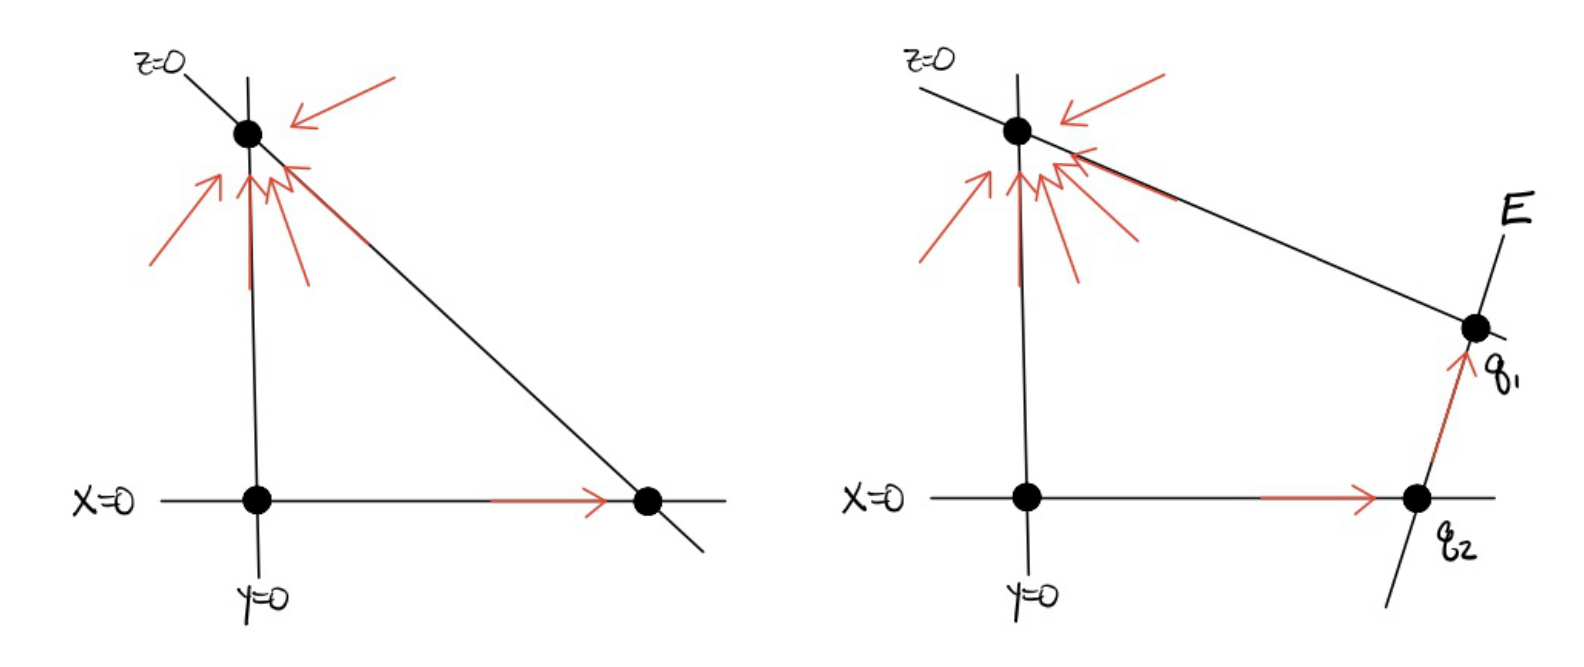
\includegraphics[width=.85\textwidth]{figures/ch07-bb-stratification.png}
\bookfiguretarget{7.8.19}
\caption{$\mathbb P^2$ (左) 与 $\operatorname{Bl}_p\mathbb P^2$ (右) 的 Białynicki--Birula 分层.}\bookfigurehref{7.8.19}\label{src:7.8.19}
\end{figure}

\subsection{Białynicki--Birula 分层在上同调中的应用}\label{src:7.8.4-subsection}
\begin{proposition}\label{src:7.8.20}
设 $X$ 是代数闭域 $\Bbbk$ 上光滑, 不可约, 拟射影的概形, 带有仅有有限个不动点的 $\mathbb G_m$-作用. 则 $\mathrm{CH}_i(X)$ 是由 $i$ 维胞腔的闭包生成的自由 $\mathbb Z$-模. 若 $\Bbbk=\mathbb C$, 则到 Borel--Moore 同调的循环映射 $\mathrm{CH}_i(X)\to H_{2i}^{\mathrm{BM}}(X,\mathbb Z)$ 是同构, 且 $H_{2i+1}^{\mathrm{BM}}(X,\mathbb Z)=0$.
\end{proposition}
\begin{remark}\label{src:7.8.21}
$X$ 紧致时 (如射影时), $H_{2i}^{\mathrm{BM}}(X,\mathbb Z)$ 就是通常的整系数奇异同调.
\end{remark}
\begin{proof}
Białynicki--Birula 分层~\bookref{7.8.14}(4) 说明 $X$ 有胞腔分解, 结论来自 \cite[例 19.1.11]{Ful98}. 另见 \cite[\S3.2]{Bri97}.
\end{proof}
\begin{example}[$\Hilb^n(\mathbb A^2)$ 的 Chow 群]\label{src:7.8.22}
令 $X=\Hilb^n(\mathbb A^2)$ 为 $n$ 个点的 Hilbert 概形, 它光滑不可约 (见 \bookref{2.5.3}). 自然的 $\mathbb G_m^2$-作用诱导 $X$ 上的作用. 在 $\mathbb G_m\to\mathbb G_m^2$, $t\mapsto(t,t)$ 诱导的作用下, 取值映射 $\operatorname{ev}_0:X^+\to X$ 满射, 且 $\mathbb G_m$-不动点对应于支撑在原点, 由单项式理想 $I$ 定义的子概形 $Z=V(I)\subseteq\mathbb A^2$, 因而只有有限个不动点. 可用命题~\bookref{7.8.20} 计算 $\mathrm{CH}^*(X)$.

对单项式理想 $I\subseteq R:=\Bbbk[x,y]$ 及 $i\ge0$, 定义 $a_i:=\min\{j\mid x^iy^j\in I\}$, 令 $r$ 为使 $a_r>0$ 的最大整数. 则 $a_0\ge\cdots\ge a_r$ 是 $n$ 的分拆, $I=(y^{a_0},xy^{a_1},\ldots,x^{r+1})$. 要计算 $\mathbb G_m$ 在单项式理想处切空间 $T_I=\Hom_R(I,R/I)$ 上的正权重空间 $T_{I,>0}$ 的维数. 此切空间由习题~\bookref{2.5.6} 与 $\Hom_R(I,R/I)$ 等同. 先证明作为 $\mathbb G_m^2$-表示有
\begin{align}\label{src:7.8.23}
T_I=\sum_{0\le i\le j\le r}\sum_{s=a_{j+1}}^{a_j-1}\bigl(\chi_1^{i-j-1}\chi_2^{a_i-s-1}+\chi_1^{j-i}\chi_2^{s-a_i}\bigr),
\end{align}
其中 $\chi_i:\mathbb G_m^2\to\mathbb G_m$ 为 $(t_1,t_2)\mapsto t_i^{-1}$ 给出的一维表示. 右侧出现
\begin{align*}
\sum_{0\le i\le j\le r}2(a_j-a_{j+1})=2\sum_{0\le i\le r}a_i=2n=\dim T_I
\end{align*}
个一维表示, 且线性无关. 只需证明每个都出现于 $T_I$. $R$-模映射 $\phi:I\to R/I$ 由 $\phi(x^iy^{a_i})$ 决定, 满足关系
\begin{align*}
\phi(x^{i+1}y^{a_i})=x\phi(x^iy^{a_i}),\qquad\phi(x^iy^{a_{i-1}})=y^{a_{i-1}-a_i}\phi(x^iy^{a_i}).
\end{align*}
对 $0\le i\le j\le r$, $a_{j+1}\le s<a_j$, 定义
\begin{align*}
\phi_{i,j,s}:I\to R/I,\quad x^ly^{a_l}&\longmapsto\begin{cases}x^{l+j-i}y^{a_l+s-a_i},&l\le i,\\0,&\text{其他情形},\end{cases}\\
\psi_{i,j,s}:I\to R/I,\quad x^ly^{a_l}&\longmapsto\begin{cases}x^{l+i-j-1}y^{a_l+s-a_i},&l\ge j+1,\\0,&\text{其他情形}.\end{cases}
\end{align*}
可检验它们是 $R$-模映射, 分别为 $\chi_1^{j-i}\chi_2^{s-a_i}$ 与 $\chi_1^{i-j-1}\chi_2^{a_i-s-1}$ 的特征向量, 故 \bookeqref{7.8.23} 成立.

取 $\lambda=(\lambda_1,\lambda_2):\mathbb G_m\to\mathbb G_m^2$, $\lambda_1\gg\lambda_2$. 按我们的符号约定, \bookeqref{7.8.23} 中特征标 $\chi_1^a\chi_2^b$ 关于 $\lambda$ 的权重为正, 当且仅当 $a<0$, 或 $a=0,b<0$. 因而
\begin{align*}
T_{I,>0}=\sum_{0\le i\le j\le r}\sum_{s=a_{j+1}}^{a_j-1}\chi_1^{i-j-1}\chi_2^{a_i-s-1}+\sum_{j=0}^r\sum_{s=a_{j+1}}^{a_j-1}\chi_1^{j-i}\chi_2^{s-a_i},
\end{align*}
且
\begin{align*}
\dim T_{I,>0}&=\Bigl(\sum_{i=0}^r\sum_{j=i}^r(a_j-a_{j+1})\Bigr)+\Bigl(\sum_{j=0}^r(a_j-a_{j+1})\Bigr)\\
&=\Bigl(\sum_{i=0}^ra_i\Bigr)+a_0=n+a_0.
\end{align*}
因满足 $\dim_{\Bbbk}R/I=n$ 的单项式理想与 $n$ 的分拆 $a_0\ge\cdots\ge a_r$ 双射, 对每个 $d\ge0$, 满足 $\dim T_{I,>0}=d$ 的单项式理想个数等于
\begin{align}\label{src:7.8.24}
P(2n-d,d-n):=\#\{2n-d\text{ 的分拆 }a_1\ge\cdots\ge a_r\mid a_i\le d-n\}.
\end{align}
由命题~\bookref{7.8.20}, 得 $\dim\mathrm{CH}_d(\Hilb^n(\mathbb A^2))_{\mathbb Q}=P(2n-d,d-n)$. 另见 \cite[定理 1.1]{ES87} 与 \cite[\S2.2]{Göt94}.
\end{example}
\begin{exercise}[$\Hilb^n(\mathbb P^2)$ 的 Chow 群]\label{src:7.8.25}
依照上述策略证明 $\Hilb^n(\mathbb P^2)$ 的第 $d$ 个 Betti 数 $b_d$ (等价地, $\dim\mathrm{CH}_d(\Hilb^n(\mathbb P^2))$) 等于
\begin{align*}
b_d=\sum_{n_0+n_1+n_2=n}\sum_{p+r=d-n_1}P(p,n_0-p)P(n_1)P(2n_2-r,r-n_2),
\end{align*}
其中 $P(a)$ 为 $a$ 的分拆数, $P(a,b)$ 由 \bookeqref{7.8.24} 定义.
\end{exercise}
\begin{remark}\label{src:7.8.26}
Göttsche 在 \cite[定理 0.1]{Göt90} 中利用 Weil 猜想 (另见 \cite[定理 2.3.10]{Göt94}), 证明 $\mathbb C$ 或 $\overline{\mathbb F}_q$ 上任意光滑射影曲面 $S$ 的 $S^{[n]}:=\Hilb^n(S)$ 的 Poincaré 多项式 $p(S^{[n]},z)=\sum_i b_i(S^{[n]})z^n$ 满足
\begin{align*}
\sum_{n=0}^{\infty}p(S^{[n]},z)t^n
=\prod_{m=1}^{\infty}\frac{(1+z^{2m-1}t^m)^{b_1(S)}(1+z^{2m+1}t^m)^{b_3(S)}}{(1-z^{2m-2}t^m)^{b_0(S)}(1-z^{2m}t^m)^{b_2(S)}(1-z^{2m+2}t^m)^{b_4(S)}}.
\end{align*}
特别地, $S^{[n]}$ 的 Betti 数只依赖 $S$ 的 Betti 数. 各个 $p(S^{[n]},z)$ 未必有特别好的表达式, 但涉及所有 $n$ 的生成函数有. 另一方面, Nakajima 构造了 Heisenberg 代数在 $H_*(S^{[n]})$ 上的作用, 可用于恢复上述公式及上同调环的更多性质 \cite{Nak97} (另见 \cite{Nak99b}).
\end{remark}
Białynicki--Birula 分层也可用于计算等变 Chow 环 $\mathrm{CH}_G^*(X)$; 见习题~\bookref{8.7.12}.
